\section{Epilepsy}

% What it is, prevalence
Epilepsy is a neurological condition characterized by abnormal brain activity that gives rise to recurring seizures, affecting about 600 000 people in the UK and 50 million people worldwide \cite{nice_epilepsies_2012,fiest_prevalence_2017}.
This means that around 1\% of the world population live with epilepsy.

% Personal and global burden
Epilepsy is associated with "stigma, psychiatric comorbidity, and high economic costs", and it has been ranked by the \ac{WHO} as the second most burdensome neurological disorder in terms of disability-adjusted life years \cite{fiest_prevalence_2017}.
% Deaths in the UK/SUDEP
There are 21 epilepsy-related deaths in the UK every week%
\fnurl{https://sudep.org/epilepsy-deaths}.
Around half of these deaths are \ac{SUDEP}.  % 600/year -> 11.5/week, according to https://epilepsysociety.org.uk/living-epilepsy/sudden-unexpected-death-epilepsy-sudep
\ac{SUDEP} is more formally defined as ``the sudden, unexpected, witnessed or unwitnessed, non-traumatic, and non-drowning death in patients with epilepsy with or without evidence for a seizure, and excluding documented status epilepticus, in which postmortem examination does not reveal a structural or toxicological cause for death'' \cite{nashef_sudden_1997}.
It is the most common category of epilepsy-related deaths \cite{devinsky_sudden_2016}.
The underlying mechanisms of \ac{SUDEP} are not fully understood, and looking for patterns to predict its risk is an active research field \cite{so_what_2008,alexandre_risk_2015,vilella_association_2021,jha_sudden_2021}.

Antiepileptic drugs are normally used to treat epilepsy.
However, in roughly one third of the patients, antiepileptic drugs do not adequately control seizures.
These patients are described as being medically refractory.
Half of the medically refractory epileptic patients have focal epilepsy, which may be treated by curative resective surgery.


% \subsection{Assessment for epilepsy surgery}

The objective of resective epilepsy surgery is the complete resection or complete disconnection of the \ac{EZ}, which is defined as ``the area of cortex indispensable for the generation of clinical seizures'' \cite{rosenow_presurgical_2001}.
The surgery is performed if the \ac{EZ} can be definitely identified and is located in a part of the brain that may be removed without causing neurological, cognitive or neuropsychiatric deficit \cite{jobst_resective_2015}.

To locate the \ac{EZ}, several preoperative imaging scans such as \ac{T1w} \acp{MRI} are acquired in order to identify structural cerebral abnormalities, such as hippocampal sclerosis \cite{thom_review_2014} or focal cortical dysplasia \cite{kabat_focal_2012}.
Hippocampal sclerosis refers to the loss of neurons and gliosis within the hippocampus.
It is characterised by the hippocampus shrinking and increased signal intensity on \ac{T1w} \ac{MRI}.
Dysplasia is one of a range of malformations of cortical development with malalignment of the normal 6-layer cerebral cortex and, in some cases, morphologically abnormal neurons and glia, and dysmyelination.
Focal cortical dysplasia is characterised as a thickening or structural abnormality in the cortical gray matter.
\cref{fig:lesions} shows an image from an epileptic patient with focal cortical dysplasia with ipsilateral hippocampal sclerosis%
\footnote{The coexistence of hippocampal sclerosis and focal cortical dysplasia is not very common.
About 15\% of patients with hippocampal sclerosis have a co-existent neocortical pathology, e.g.\ glioma, dysembryoplastic neuroepithelial tumour, cortical dysplasia or cavernoma}.
Video \ac{EEG} telemetry is also routinely done over several days to record the patient's brain activity.

\begin{figure}
  \centering
  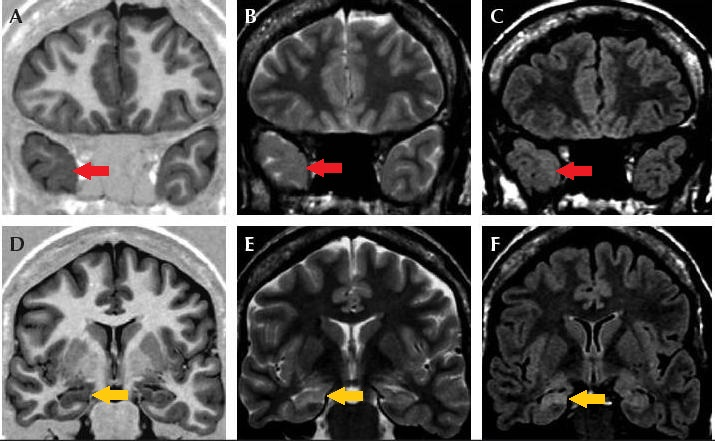
\includegraphics[width=\linewidth]{figures/lesions_arrows}
  \caption[Focal cortical dysplasia with ipsilateral hippocampal sclerosis]{
    Focal cortical dysplasia with ipsilateral hippocampal sclerosis.
    The images are coronal slices at the level of the temporal pole (top) and the head of the hippocampus (bottom).
    They are presented in radiological convention, i.e.\ the patient right side is on the left side of the screen and vice versa. A, D: turbo spin-echo inversion-recovery $T_1$-weighted; B,E: turbo spin-echo $T_2$-weighted; C, F: turbo spin-echo FLAIR $T_2$-weighted.
    Red arrows point to a hypoplasia of the right temporal pole with volume loss of the white matter which leads to mild hyperintensity on $T_2$-weighted images; mild blurring of the cortical-white matter junction is visible on both $T_1$- and $T_2$-weighted images (A–C).
    Yellow arrows point to the atrophic hippocampus, with a decreased signal on IR-$T_1$-weighted images and increased signal on $T_2$-weighted images, consistent with hippocampal sclerosis.
    Courtesy of \cite{colombo_imaging_2009}.
  }
  \label{fig:lesions}
\end{figure}
